\section{Cypher}
A linguagem utilizada para trabalhar com o Neo4j chama-se Cypher, a primeira representação que devemos conhecer é:
\begin{itemize}[nolistsep]
	\item \textbf{Parênteses} devem ser usados para os nós.
	\item \textbf{Chaves} devem ser usadas para as propriedades.
	\item \textbf{Colchetes} devem ser usados para os relacionamentos.
\end{itemize}

Uma dica simples podemos tentar comparar com os comandos SQL, porém essa linguagem nada tem a ver, por exemplo, um comando básico usado frequentemente é:
\begin{lstlisting}[]
MATCH (a)-[:DONA]->(b) RETURN a, b;
\end{lstlisting}

Realiza uma consulta que mostra como obter todos os nós que estão relacionados entre si por um determinado relacionamento chamado \textbf{DONA}. Mas vamos começar com muita calma e ir avançado, para executar qualquer comando, na barra de comandos do \textit{Neoj Browser} digitamos:
\begin{lstlisting}[]
MATCH (n) RETURN n;
\end{lstlisting}

E pressionamos o botão para executar, o resultado deve ser algo assim:
\begin{figure}[H]
	\centering
	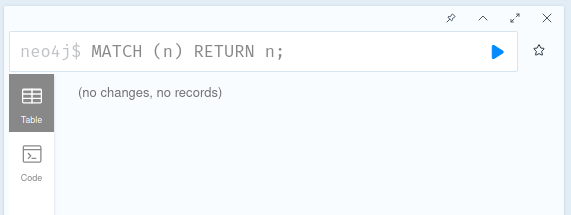
\includegraphics[width=0.4\textwidth]{imagens/consulta}
	\caption{Execução do comando no Neo4j Browser}
\end{figure}

Essa consulta nos mostra que não existe nenhum banco ou registro cadastrado. Em seguida, veremos uma estrutura completa do banco de dados, para facilitar o entendimento tentaremos associar isso aos comandos SQL.

\subsection{Comando CREATE / CREATE UNIQUE}
Este comando é utilizado para criarmos qualquer elemento no banco de dados: nós, relacionamentos, propriedades ou combinações entre eles. Podemos associá-lo com \textbf{INSERT}, porém age de forma bem diferente do SQL, primeiro um Nó (que seria o correspondente a uma entidade) pode ter vários nomes, por exemplo:
\begin{lstlisting}[]
CREATE (:Pessoa:Proprietario);
\end{lstlisting}

Podemos criar algumas propriedades para este nó:
\begin{lstlisting}[]
CREATE (:Pessoa { nome : 'Fernando', modelo_carteira : "AB" });
CREATE (:Pessoa { nome : 'Anselmo', modelo_carteira : "B" });
CREATE (:Automovel { nome : 'Ecosport' });
\end{lstlisting}

Os relacionamentos são criados assim, para a pessoa com o nome "Fernando":
\begin{lstlisting}[]
MATCH (p:Pessoa { nome: "Fernando" }) OPTIONAL MATCH (a:Automovel { nome: "Ecosport" }) CREATE (p)-[:DONA]->(a)
\end{lstlisting}

E para a pessoa com o nome "Anselmo":
\begin{lstlisting}[]
MATCH (p:Pessoa { nome: "Anselmo" }) OPTIONAL MATCH (a:Automovel { nome: "Ecosport" }) CREATE (p)-[:DONA]->(a)
\end{lstlisting}

E com o comando:
\begin{lstlisting}[]
MATCH (n) RETURN n;
\end{lstlisting}

Podemos visualizar o seguinte Grafo:
\begin{figure}[H]
	\centering
	\includegraphics[width=0.3\textwidth]{imagens/relacionamento}
	\caption{Grafo entre Pessoa e Automóvel}
\end{figure}

Também podemos criar simultaneamente todas as pessoas e seus relacionamentos com um único comando que seria:
\begin{lstlisting}[]
CREATE (:Pessoa {nome: "Fernando", modelo_carteira : "AB"})-[:DONA]->(:Automovel {nome: "Ecosport"})<-[:DONA]-(:Pessoa {nome: "Anselmo", modelo_carteira : "B"});
\end{lstlisting}

\subsection{Comando MATCH - Subcomando SET}
Normalmente o comando \textbf{MATCH} é associado com o \textbf{SELECT}, porém faz muito mais já o vimos associado ao \textbf{CREATE}, com sua associação a SET podemos adicionar ou criar propriedades nos nós:
\begin{lstlisting}[]
MATCH (n) WHERE n.nome = "Fernando" SET n.profissao = "Desenvolvedor"
\end{lstlisting}

Se reparar na sintaxe podemos fazer uma associação ao comando \textbf{UPDATE}.

\subsection{Comando MATCH - Para consultas}
Nota-se que este é o principal comando em Cypher, o comando MATCH é extremamente versátil, para retornarmos todas as pessoas com um nome específico:
\begin{lstlisting}[]
MATCH (n:Pessoa {nome: "Fernando"}) RETURN n;
\end{lstlisting}

Retornar um conjunto específico de propriedades (não todas):
\begin{lstlisting}[]
MATCH (p:Pessoa {nome: "Fernando"})
RETURN p.modelo_carteira, p.profissao
\end{lstlisting}

Retornar todas as pessoas que não possuem o valor de alguma propriedade específica:
\begin{lstlisting}[]
MATCH (p:Pessoa) 
WHERE NOT p.nome = 'Anselmo'
RETURN j
\end{lstlisting}

A subcláusula WHERE funciona quase da mesma forma que o SQL, por exemplo, vamos supor que as pessoas tivessem uma propriedade "experiencia" (em anos) e desejamos conhecer todas em um determinado intervalo:
\begin{lstlisting}[]
MATCH (p:Pessoa)
WHERE 3 <= p.experiencia <= 7
RETURN p
\end{lstlisting}

Ou para avaliar a existência de um determinado valor em um relacionamo:
\begin{lstlisting}[]
MATCH (p:Pessoa)-[rel:DONA]->(a:Automovel)
WHERE p.modelo_carteira IS NOT NULL
RETURN p, rel, a;
\end{lstlisting}

Para combinarmos os nós que estão relacionados, independentemente da direção (observe a falta de uma seta) e retornar de ambos os lados:
\begin{lstlisting}[]
MATCH (a)--(b) RETURN a, b;
\end{lstlisting}

Podemos atribuir os relacionamentos a uma variável "r", e isso significa que podem ser retornados da consulta, portanto, se precisamos do relacionamento (ou qualquer uma de suas propriedades):
\begin{lstlisting}[]
MATCH (a)-[r]-(b) RETURN a, r, b;
\end{lstlisting}

Quando não desejamos caracterizar tudo, ou seja somente um certo tipo de relacionamento, adicionamos o padrão ":TIPO". Nesse caso, o tipo é DONA e, como o relacionamento não é necessário posteriormente, o alias é descartado:
\begin{lstlisting}[]
MATCH (a)-[:DONA]->(b) RETURN a, b;
\end{lstlisting}

Em vez de apenas retornar todos os nós envolvidos em um caminho, podemos obter o próprio caminho. Com base no exemplo anterior, isso será transformado em um caminho nomeado:
\begin{lstlisting}[]
MATCH p=(a)-[:DONA]->(b) RETURN p;	
\end{lstlisting}

É possível usar várias cláusulas MATCH em uma consulta, portanto, para retornar dois nós específicos, podemos usar várias causas de correspondência e, em seguida, retornar o resultado: 
\begin{lstlisting}[]
MATCH (a:Pessoa {nome: 'Fernando'})
MATCH (b:Pessoa {nome: 'Anselmo'})
RETURN a, b;
\end{lstlisting}

Que podemos simplificar para:
\begin{lstlisting}[]
MATCH (a:Pessoa {nome: 'Fernando'}),(b:Pessoa {nome: 'Anselmo'}) RETURN a, b;
\end{lstlisting}

Esse comando é extremamente importante pois mostra bem o princípio que discutimos sobre transações, retorna os nós solicitados exatamente como esperamos. Se o segundo MATCH falhar, então o primeiro também falha, e a consulta retorna 0 resultados, pois está procurando por um \textbf{AND} também b, portanto, caso não conseguir encontrar nada em "b" então a consulta não é válida. 

Podemos contornar isso, com a utilização de uma correspondência opcional. Retorna somente se a correspondência estiver presente. Do contrário, retornará \textbf{null}: 
\begin{lstlisting}[]
MATCH (a:Pessoa {nome: 'Fernando'})
OPTIONAL MATCH (b:Pessoa {nome: 'Anselmo'})
RETURN a, b;
\end{lstlisting}

Este sinalizador \textbf{OPTIONAL MATCH} é utilizado para retornar relacionamentos potenciais para um nó. Se apenas o nó pode ter um relacionamento, pode ser usado para remediar isso, assim: 
\begin{lstlisting}[]
MATCH (a:Pessoa {nome: 'Fernando'})
OPTIONAL MATCH (a)-->(x)
RETURN a, x;	
\end{lstlisting}

Assim para todos os nós rotulados como "Pessoa" com o nome de "Fernando", ambos os nós que possuem ou não relacionamentos serão retornados.

\subsection{Comando MATCH - Subcomando DELETE}
Vamos começar limpando nós ou relacionamentos que não possuem associações:
\begin{lstlisting}[]
MATCH (n) WHERE NOT (n)--() DELETE n
\end{lstlisting}

Observamos então que basta fazer uma consulta e usar o DELETE para eliminar o que desejamos. Por exemplo, vamos excluir um relacionamento determinado:
\begin{lstlisting}[]
MATCH (p:Pessoa {nome: "Fernando"})-[rel:DONA]->(a:Automovel {nome: "Ecosport"})
DELETE rel
\end{lstlisting}

Eliminar um nó determinado (deve estar sem relacionamentos):
\begin{lstlisting}[]
MATCH (p:Pessoa {nome: "Fernando"}) DELETE p
\end{lstlisting}

Eliminar todos com o comando (seria um correspondente a \textbf{DROP DATABASE}):
\begin{lstlisting}[]
MATCH (n) DETACH DELETE n
\end{lstlisting}

